
\section{Topología}

\begin{definicion}
    Sea $X\neq \varnothing$. Una clase $\tau$ de subconjunto de $X$ es una topología sobre $X$, se cumple: 
    \begin{enumerate}
        \item $\varnothing,X\in \tau$
        \item La unión de una clase arbitraria de conjuntos en $\tau$ es un miembro de $\tau$. 
        \item La intersección de una clase finita de miembros de $\tau$ está en $\tau$. 
    \end{enumerate}
    Los miembros de $\tau$ son los abiertos de $X$. 
\end{definicion}

\begin{cajita}
    \begin{enumerate}
        \item El par $(X,\tau)\footnotetext{estructura topológica}$ es un espacio topológico. 
        \item A los elementos de $X$ se les llama puntos. 
    \end{enumerate}
\end{cajita}

\begin{ejemplo}
    \begin{enumerate}
        \item Sea $X\neq \varnothing\implies \tau=P(X)$ es una topología sobre $X$. A $\tau$ se le llama topología discreta de $X$, y $(X,\tau)$ es un espacio discreto. 

        \item Sea $X\neq \varnothing\implies \tau =\{\varnothing,X\}$ es una topología sobre $X$. A $\tau$ se le llama topología indiscreta, y $(X,\tau)$ es un espacio indiscreto. 
        \item $X=\mathbb{R}^2$ y $\tau$ es la colección de abiertos de $\mathbb{R}^2$ definido en términos de la métrica usual. A $\tau$ se le llama topología usual de $\mathbb{R}^2$. 
        \item Sea $X=\{a,b,c,d,e\}$.
        \begin{enumerate}
            \item Sea $\tau_1=\{X,\varnothing,\{a\},\{c,d\},\{a,c,d\},\{b,c,d,e\}\}\implies \tau_1$ es una topología sobre $X$.
            \item Sea $\tau_2=\{X,\varnothing,\{a\},\{c,d\},\{a,c,d\},\{b,c,d\}\}$. Note que $\{a\}\cup \{b,c,d\}=\{a,b,c,d\}\not\in \tau_2\implies \tau_2$ no es topología sobre $X$
            \item Sea $X$ un conjunto infinito y sea $\tau$ el vacío junto con la colección de subconjunto de $X$ cuyos complementos son finitos. $\tau$ es una topología sobre $X$, y se llama topología cofinita sobre $X$. 
        \end{enumerate}  
    \end{enumerate}
\end{ejemplo}

\begin{cajita}
    \begin{nota}
        Un espacio metrizable es un espacio topológico $X$ con la propiedad que existe una métrica que genera los abiertos de la topología dada. 
    \end{nota}
    \begin{problema}
        ¿Qué tipos de espacios topológicos son metrizables?
    \end{problema}
\end{cajita}

\begin{prop}
    Si $\tau_1$ y $\tau_2$ son topologías sobre $X$, entonces $\tau_1\cap \tau_2$ es topología sobre $X$.
    \begin{dem}
        \begin{enumerate}
            \item Como $\tau_1$ y $\tau_2$ son topologías, etnonces: $X,\varnothing\in \tau_1$ y $X,\varnothing\in \tau_2\implies X\in \tau_1\cap \tau_2$ y $\varnothing\in \tau_1\cap \tau_2$. 
            \item Sea $\{G_i\}_{i\in I}$ una subcolección de $\tau_1\cap \tau_2\implies G_i\in \tau_1,\forall i\in I \implies \bigcup_i G_i\in \tau_i$ y $G_i\in \tau_2,\forall i\in I\implies\bigcup_i G_i\in \tau_2$. Entonces $\bigcup_i G_i\in \tau_1\cap \tau_2$
            \item Sea $G_1$ y $G_2\in \tau_1\cap \tau_2\implies G_1\in\tau_1$ y $G_1\in \tau_2$. $G_2\in \tau_1$ y $G_2\in \tau_2$. Entonces $G_1\cap G_2\in \tau_1$ y $G_1\cap G_2\in \tau_2\implies G_1\cap G_2\in \tau_1\cap\tau_2$. Entonces, $\tau_1\cap \tau_2$ es una topología sobre $X$. 
        \end{enumerate}
        
    \end{dem}
\end{prop}

\begin{nota}
    Sea $X=\{a,b,c\}$ y sean:
    \begin{itemize}
        \item $\tau_1=\{X,\varnothing,\{a\}\}$, $\tau_2=\{X,\varnothing, \{b\}\}$. Entonces, $\tau_1\cup \tau_2=\{X,\varnothing,\{a\},\{b\}\}$, pero $\{a,b\}\not\in \tau_1\cup\tau_2$. $\therefore\tau_1\cup\tau_2$ no es topología sobre $X$.
    \end{itemize}
\end{nota}

\begin{ejemplo}
    Sea $f:X\to Y$, donde $X$ es un conjunto no vacío y $Y$ es el espacio topológico de $(Y,\tau')$. Entonces $\tau=\{f^{-1}(G):G\in \tau'\}$ es una topología sobre $X$. En efecto:
    \begin{enumerate}
        \item $\varnothing\implies \tau'\implies f^{-1}(\varnothing)=\varnothing\in\tau$. $Y\in \tau'\implies f^{-1}(Y)=X\in\tau$
        \item Sea $\{G_i\}$ una subclase de $\tau$. Como $G_i\in \tau,\forall \implies \exists H_i\in \tau'\ni G_i=f^{-1}(H_i)\implies \cup_i G_i=\cup_{i}f^{-1}(H_i)=f^{-1}(\underbrace{\bigcup_i H_i}_{\in \tau'})\in \tau $
    \end{enumerate}
\end{ejemplo}

\begin{definicion}
    Sean $X$ y $Y$ espacios topológicos y $f$ un mapeo de $X$ en $Y$. Se dice que $f$ es continua si $f^{-1}(G)$ es un abierto de $X$ para cada abierto de $G$ de $Y$. 
\end{definicion}

\begin{definicion}
    Se dice que el mapeo es abierto si, para cada abierto $G$ de $X$, se cumple que $f(G)$ es abierto de $Y$. 
\end{definicion}

\begin{definicion}
    Si $f$ es continuo, entonces $f(x)$ es la imagen continua de $X$ bajo $f$. 
\end{definicion}

\begin{definicion}[Homeomorfismo]
    Un homeomorfismo es un mapeo biyectivo y bicontinuo (continuo y abierto) entre espacios topológicos. En este caso, los espacios son homeomorfos. 
\end{definicion}

\begin{cajita}
    \begin{nota}
        Una propiedad topológica es una propiedad que si la tiene el espacio topológico $X$, la tiene  también cualquier espacio homeomorfo a $X$
    \end{nota}
\end{cajita}


%----

\begin{nota}
    Sea $A$ un subconjunto no vacío del espacio topológico $(X,\tau)$. Considerese la clase: 
    $$\tau_A=\{A\cap G: G\in\tau \text{es abierto de $X$}\}$$
    Entonces, $\tau_A$ es una topologia sobre $A$, la cual se llama topologia relativa sobre $A$.
\end{nota}

\begin{definicion}
    El par $(A,\tau_A)$ es un espacio topologico y se dice es un subespacio de $X$, 
    \begin{enumerate}
        \item $\varnothing\in \tau\implies A\cap \varnothing=\varnothing\in\tau_A$ y $X\in \tau\implies A\cap X=A\in \tau_A$.
        \item Sea $\{G_i\}_{i\in I}$ una colección de miembros de $\tau_A\implies \exists H_i\in \tau\ni G_i=A\cap H_i, \forall i\implies \bigcup_i G_i=\bigcup_i(A\cap H_i)= A\cap\left(\underbrace{\bigcup_{i}H_i}_{\in\tau}\right)\in\tau_A$
        \item Sean $G_1,G_2\in \tau_A\implies\exists H_i\in\tau\ni G_i=A\cap H_i$, $i=1,2$. Entonces, $G_1\cap G_2=(A\cap H_1)\cap (A\cap H_2)=A\cap (\underbrace{H_1\cap H_2}_{\in\tau})\in\tau_A\implies \tau_A$ es topología sobre $A$. 
    \end{enumerate}
\end{definicion}

\begin{ejemplo}
    Tenemos, 
    \begin{enumerate}
        \item Sea $\tau$ la topología usual de $\mathbb{R}$ y considere la topología relativa $\tau_{\mathbb{Z}^+}$ (en este caso, $\mathbb{Z}^+\subset \mathbb{R})$. Nótese que $\{n
        _0\}$ es abierto, la unión de unitarios es abierto de $\tau_{\mathbb{Z}^+}\implies \tau_{\mathbb{Z}^+}$ es la topología discreta de $\mathbb{Z}^+$.
        \item Considere $(\mathbb{R},\tau)$, donde $\tau$ es la topología usual de $\mathbb{R}$ y  sea $I=[0,1]$. Entonces, 
        \begin{enumerate}
            \item $(1/2,1]=[0,1]\cap (1/2,2)\in \tau_I$
            \item $(1/2,2/3)=[0,1]\cap (1/2,2/3)\in \tau_I$
            \item $(0,1/2]\not\in \tau_I$, ya que no existe un abierto $G\in \tau\ni (0,1/2]=I\cap G$.
        \end{enumerate}
        \item Sea $X=\{a,b,c,d,e\}$ y sea 
        $$\tau=\{X,\varnothing,\{a\},\{a,b\},\{a,b,c,d\},\{a,b,e\}\}$$
        \begin{cajita}
            $\tau_A=\{A,\varnothing,\{a\},\{a,c\},\{a,e\}\}$
        \end{cajita}
        Considere $A=\{a,c,e\}$ entonces: \begin{itemize}
            \item $A\cap X=A$
            \item $A\cap\varnothing=\varnothing$
            \item $A\cap\{a\}=\{a\}$
            \item $A\cap\{a,b\}=\{a\}$
            \item $A\cap\{a,c,d\}=\{a,c\}$
            \item $A\cap \{a,b,c,d\}=\{a,c\}$
            \item $A\cap\{a,b,e\}=\{a,e\}$
        \end{itemize}
    \end{enumerate}
\end{ejemplo}

%---------
\subsubsection{Objeto de estudio de la topología}: Estudio de todas las propiedades topológicas de los espacios

\begin{definicion}
    Sea $(X,\tau)$ un espacio topológico. Un subconjunto $A\subset X$ es cerrado si y solo si $A^c\in\tau $.
\end{definicion}

\begin{ejemplo}
    Sea $(X,\tau)$ un espacio discreto. Sea $A\subset X\implies A\in\tau\implies A^c\subset X\implies A^c\in \tau\implies A$ es cerrado. Entonces, $A\subset X$ es abierto y cerrado en $X$. 
\end{ejemplo}

\begin{cajita}
    \begin{nota}
        Sea $(X,\tau)$ un espacio topológico,
        \begin{enumerate}
            \item $\phi\in \tau\implies \phi^c=X$ es cerrado. $X\in\tau\implies X^c=\phi$ es cerrado.
            \item Considere una familia arbitraria $\{F_i\}$ de cerrados en $\tau\implies \{F_i^c\}\subset \tau\implies \bigcup_i F_i^c\in \tau \implies \left(\bigcup_i F_i^c\right)^c=\bigcap_i F_i$ es cerrado. 
            \item Sean $F_1$ y $F_2$ cerrados en $\tau\implies F_1^c$ y $F_2^c\in\tau\implies F_1^c\cap F_2^c\in \tau\implies (F_1^c\cap F_2^c)^c=F_1\cup F_2$ es cerrado.   
        \end{enumerate}
    \end{nota}
\end{cajita}


\begin{definicion}
    Sea $X$ un espacio topológico: 
    \begin{enumerate}
        \item Una vecindad de un punto (o de un conjunto), es un abierto de $X$ que contiene al punto (o al conjunto).
        \item Sea $A\subseteq X$. Un punto $x$ en $A$ es aislado si existe una vecindad de $x$ que no contiene ningún otro punto de $A$. 
        \item Sea $A\subseteq X$. Un punto de $y\in X$ es un punto límite de $A$ si, $\forall G\in \tau\ni y\in G$, se tiene que $(G-\{y\})\cap A\neq\varnothing$. 
        \begin{cajita}
            EL conjunto de puntos límite de $A$ se llama derivado de $A$, $(A',D(A))$.  
        \end{cajita}
        \item Sea $A\subseteq X$. La cerradura de $A$, denotado $\overline{A}$, es el cerrado más pequeño que contiene a $A$. Es decir, si $F_i$ son los cerrados de $X$ que contiene a $A\implies \overline{A}=\bigcap_i F_i$. 
        \begin{cajita}
            Tenemos:
            \begin{enumerate}
                \item $A\subseteq \overline{A}$
                \item Si $A$ es cerrado $\implies A=\overline{A}$.
            \end{enumerate}
        \end{cajita}
        \item Un subconjunto $A$ de $X$ es denso (siempre denso), si $\overline{A}=X$.
        \item El espacio topológico $X$ es separable si tiene un subconjunto separable contable y denso. 
        \item Un punto de adherencia de $A\subseteq X$ es cualquier elemento de $\overline{A}$.
    \end{enumerate}
\end{definicion}

\begin{prop}
    Sea $A\subset B\implies A'\subset B'$.
    \begin{prop}
        Sea $A\subset B$ y sea $x\in A'\implies$ si $G$ es un abierto $\ni x\in G\implies (G-\{x\})\cap B\supset (G-\{x\})\cap A\neq \varnothing\implies x\in B'\implies A'\subset B'$.
    \end{prop}
\end{prop}

\begin{prop}
    Derivado de la unión $(A\cup B)'=A'\cup B' $
    \begin{dem}
        Por doble contención:
        \begin{itemize}
            \item $(\supseteq)$. A probar: $A'\cup B'\subset (A\cup B)'$. Sea $A\subseteq A\cup B$ y $B\subseteq A\cup B\implies A'\subseteq (A\cup B)'$ y $B'\subseteq (A\cup B)'\implies A'\cup B'\subseteq (A\cup B)'$
            \item $(\subseteq)$. A probar $(A\cup B)'\subseteq A'\cup B'\iff x\in (A\cup B)'\implies x\in A'\cup B'\iff$ si $x\not\in A'\cup B'\implies x\not\in (A\cup B)'$.
            \begin{itemize}
                \item Suponemos que $x\not\in A'\cup B'\implies x\not\in A'$ y $x\not\in B'\implies$ existen $G,H$ abiertos de $X\ni x\in G$ y $x\in H$ y $(G-\{x\})\cap A=\varnothing$ y $(H-\{x\})\cap B=\varnothing $ ya que $x\in G$ y $x\in H\implies x\in G\cap H$. Además, $G\cap H\subseteq G$ y $G\cap H\subseteq H$. Entonces $(G\cap H-\{x\})\cap A=\varnothing$ y $(G\cap H-\{x\})\cap B =\varnothing$. Por lo tanto, $(G\cap H-\{x\})\cap (A\cup B)=\varnothing$. 
            \end{itemize}
        \end{itemize}
    \end{dem}
\end{prop}
\begin{prop}
    $A\subseteq X$ es cerrado ssi $A'\subseteq A$.
    \begin{dem}
        Sea
        \begin{itemize}
            \item $(\implies)$
            \item $(\impliedby)$
        \end{itemize}
    \end{dem}
\end{prop}

\begin{prop}
    Sea $F$ un superconjunto cerrado de $A$, entonces $A'\subset F$. 
    \begin{dem}
        Como $A\subset F\implies A'\subset F'$. Como $F$ es cerrado, $F'\subset F\implies A'\subset F$.
    \end{dem}
\end{prop}

\begin{prop}
    $A\cup A'$ es cerrado.
    \begin{dem}
        A probar: $(A\cup A')^c$ es abierto. Sea $x\in (A\cup A')^c\implies x\not\in A$ y $x\not\in A'\implies \exists G$ abierto $\ni G\cap A=\varnothing$. 
        \begin{cajita}
            Sea $G\cap A'=\varnothing$. Supóngase que $y\in G\cap A'\implies y \in G$ y $y\in A'\implies (G-\{y\})\cap A\neq 0(\to\gets)$
        \end{cajita}
        Por otra parte, $G\cap A'=\varnothing$. Entonces, 
        \begin{align*}
            G\cap (A\cup A') &= (G\cap A)\cup (G\cap A')\\
            &= \varnothing \cup \varnothing\\
            &= \varnothing
        \end{align*}
        $\implies G\subset (A\cup A')^c\implies (A\cup A')^c$ es abierto $\implies A\cup A'$ es cerrado. 
    \end{dem}
\end{prop}


\begin{prop}
    $\overline{A}=A\cup A'$
    \begin{dem}
        Sea \begin{itemize}
            \item A probar $\overline{A}\subset A\cup A'\implies A\subset \underbrace{A}_{cerrado}\cup A'\implies A\subset \overline{A}\subset A\cup \overline{A}$.
            \item A probar: $A\cup A'\subset \overline{A}$. Entonces $A\subset \overline{A}$, $A'\subset (\overline{A})'\subset \overline{A}$. Entonces $A\subset\overline{A}$ y $\overline{A}\subset \overline{A}$, entonces $A\cup A'\subset \overline{A}$.
        \end{itemize}
    \end{dem}
\end{prop}


\begin{prop}
    Si $A\subset B\implies \overline{A}\subset \overline{B}$.
    \begin{dem}
        $A\subset B\implies A'\subset B'\implies A\cup A'\subset B\cup B'\implies \overline{A}\subset \overline{B}$. 
    \end{dem}
\end{prop}

\begin{prop}
    $\overline{A\cup B}=\underbrace{\overline{A}\cup \overline{B}}_{cerrado}$
    \begin{dem}
        \begin{itemize}
            \item Sabemos que $A\cup B\subset \overline{A}\cup \overline{B}\implies A\cup \subset \overline{A\cup B}\subset \overline{A}\cup \overline{B}.$
            \item $A\subset A\cup B\implies \overline{A}\subset \overline{A\cup B}$ y $B\subset A\cup B\implies \overline{B}\subset \overline{A\cup B}$. Entones $\overline{A}\cup\overline{B}\subset \overline{A\cup B}$
        \end{itemize}
    \end{dem}
\end{prop}

\begin{teorema}
    Sea \begin{enumerate}
        \item $\overline{\varnothing}=\varnothing$
        \item $A\subset \overline{A}$
        \item $\overline{A\cup B}=\overline{A}\cup \overline{B}$
        \item $\overline{\overline{A}}=\overline{A}$
    \end{enumerate}


    \begin{dem}
        \begin{enumerate}
            \item Como $\varnothing$ es cerraddo entonces $\overline{\varnothing}=\varnothing$
            \item $A\subset \overline{A}$, por la cerradura. 
            \item $\overline{A\cup B}=\overline{A}\cup \overline{B}$, por propiedad anterior. 
            \item Como $\overline{A}$ es cerrado, entonces $\overline{\overline{A}}=\overline{A}$.
        \end{enumerate}
    \end{dem}
    
\end{teorema}

\begin{definicion}
    \begin{enumerate}
        \item Un punto $P$ de $X$ es interior de $A\subseteq X$, si existe un abierto $G\ni$
        $$p\in G\subset A$$
        \item El interior de $A$, denotado $\int(A)$ o $A^{\circ}$, es el conjunto de todos los puntos interiores de $A$. 
    \end{enumerate}
    
\end{definicion}
\begin{definicion}
    Un punto frontera de $A\subset X$ es un punto tal que, cada vecindad del punto intersecta a $A$ y $A^c$.
\end{definicion}

 
\section{Bases y subases de una topología}

\begin{definicion}
    Una base $\beta$ (abierta) para el espacio topológico $(X,\tau)$ es una clase de abiertos de $X$ tal que cada abierto en $\tau$ puede escribirse como uniones de los miembros de la clase. 
\end{definicion}

\begin{ejemplo}
    Sea $(X,\tau)$ un espacio discreto. Entonces $\beta = \{\{x\}:x\in X\}$ es una base para $\tau$
\end{ejemplo}

\begin{cajita}
    \begin{nota}
        \begin{enumerate}
            \item Si cada $G\in \tau$ puede representarse como $G=\bigcup_iB_i$, donde $B_i\in \beta\implies$ para cada $x\in G\implies x\in B_{i_0},$ (miembro de la unión) para algún $i_0$. $\implies x\in B_{i_0}\subseteq \bigcup_i B_i=G$
        \end{enumerate}
    \end{nota}
\end{cajita}

\begin{definicion}
    Sea $(X,\tau)$ un espacio topológico. Una subclase $S$ de abiertos en $\tau$ es una subbase de la topología $\tau$, si las intersecciones finitas de miembros de $S$ producen una base $\tau$. 
\end{definicion}

\begin{ejemplo}
    \begin{enumerate}
        \item Sean $a,b\in\mathbb{R}\ni a<b$. Nótese que 
        $$(a,b)\subseteq \mathbb{R}$$
        \item ejemplo 2
        \item Sea $a=\{\{a\}\}$, entonces $\beta=\{\{a\},X\}\implies \tau=\{X,\varnothing,\{a\}\}$
        \item $a=\{\varnothing\}\implies \beta=\{X,\varnothing\}\implies \tau=\{X,\varnothing\}$
    \end{enumerate}
    
\end{ejemplo}
\begin{teorema}
    Los enunciados siguientes son equivalentes:
    \begin{enumerate}
        \item Una familia $\beta$ de subconjuntos abiertos del espacio topológico $(X,\tau)$ es una base para $\tau$, si cada abierto de $\tau$ es unión de miembros de $\beta$.
        \item $\beta\subset \tau$ es una base para $\tau$ ssi $\forall G\in \tau,\forall p\in G\exists B_p\in \beta \ni p\in B_p\subset G$.
    \end{enumerate}
    \begin{dem}
        \begin{itemize}
            \item $(i)\to(ii)$ Sea $G\in \tau$ y sea $p\in G$. Como $G\in\tau$ y $\beta$ es base de $\tau\implies G=\bigcup_iB_i,B_i\in \beta$. Como $p\in G\implies p \in \bigcup_i B_i\implies \exists i_p\ni p\in B_{i_p}\implies $ dado $p\in G\exists B_{i_p}\in \beta \ni p\in B_{i_p}\subset G$. 
            \item $(ii)\to (i)$ Sea $G\in \tau\implies$ Para cada $x\in G\exists B_x=\beta \ni x\in B_x\subset G\implies \bigcup_{x\in G}=G\implies$ es union de miembros de $\beta$.  
        \end{itemize}
    \end{dem}
\end{teorema}
\begin{teorema}
    Sea $\beta$ una familia de subconjuntos de un conjunto no vacío $X$. Entonces, $\beta$ es una base para una topologia $\tau$ sobre $X$ ssi se cumplen: 
    \begin{enumerate}
        \item $X=\bigcup_{B\in\beta}B$
        \item $\forall B,B^*\in \beta$ se tiene que $B\cap B^*$ la union de miembros de $\beta(\iff p\in B\cap B^*\exists B_p\in \beta \ni p\in B_p\subset B\cap B^*)$
    \end{enumerate}
    \begin{dem}
        \begin{itemize}
            \item $(\to)$ Sea $\beta$ la base de una topologia $\tau$ sobre $X$. Sabemos que $X$ es abierto $\implies X=\bigcup_{B\in \beta}B$, donde esta union se toma sobre todos los miembros de $\beta$. Como $\beta$ es base para $\tau\implies B\cap B^*$ puede escribirse como union de miembros de $\beta$. 
            \item $(\gets)$ Sea $\tau$ la colección de las uniones de miembros de la familia de subconjuntos de $X$. A probar: $\tau$ es topologia. 
            \begin{enumerate}
                \item Por (i) $X\in \tau$. Además, la union de la clase vacia de $\beta$ es $\varnothing\implies \varnothing\in \tau$. 
                \item Sea $\{G_i\}_{i\in I}$ una familia de miembros de $\tau$. Entonces, $G_i =\bigcup_{B\in\beta}B_{G_i}$ (donde cada $G_i$ es union de miembros de $\beta$) $\implies \bigcup_i$ es union de uniones de miembros de $\beta\implies \bigcup_i G_i\in \tau$. 
                \item Sean $G_1,G_2\in \tau\implies G_i=\bigcup\{B_i:i\in I\}$ y $G_2=\bigcup \{B_j:j\in J\}$. Entonces, $G_1\cap G_2=(\bigcup_i B_i)\cap (\bigcup_j B_j)=\bigcup_{i=j}(B_i\cap B_j)\implies G_1\cap G_2\in \tau\implies\tau$ es una topologia sobre $X$. 
            \end{enumerate}
        \end{itemize}
    \end{dem}
\end{teorema}

\begin{ejemplo}
    Sean $(a_1,b_1)$ y $(a_2,b_2)$ intervalos abiertos y acotados de $\mathbb{R}\implies$

    \begin{align}
        (a_1,b_1)\times (a_2,b_2)\left\{(x,y)\in \mathbb{R}^2,a_1<x<b_1,a_2<y<b_2\right\}
    \end{align}
\end{ejemplo}

\begin{teorema}
    Sea $X$ cualquier conjunto no vacío y sea $S$ una clase arbitraria de subconjuntos de $X$. Entonces, $S$ puede constituirse en la subbase para una topología abierta para una topología sobre $X$ en el sentido que las intersecciones finitas de los miembros de $S$ producen una base para dicha topología. 
\end{teorema}

\begin{teorema}
    Sea $X\neq \varnothing$ y sea $S$ una clase arbitraria de subconjunto de $X$. Entonces, $S$ puede servir como subbase abierta de una topología sobre $X$ en el sentido que la clase $\tau$ de todas las uniones de intersecciones finitas en $S$ es una topogía. 
    \begin{dem}
        Tenemos:
        \begin{enumerate}
            \item $S=\varnothing\implies \beta =\{X\}\implies \tau=\{X,\varnothing\}$ es la topología indiscreta.
            \item $S\neq \varnothing$l. A probar: $\tau$ es topología. 
            \begin{enumerate}
                \item $\varnothing, X\in \tau $
                \item $\{G_i\}_{i\in I}$ una subclase arbitraria de $\tau$. A probar: $\bigcup_i G_i\in \tau$. Cada $G_i$ es unión de intersecciones finitas de miembros de $S$. Entonces, $\bigcup_i G_i$ es unión de uniones de intersecciones finitas de miembros de $S \implies \bigcup_i G_i\in \tau$. 
                \item Sea $G_1,G_2\in \tau$. A probar $G_1\cap G_2\in \tau$. $G_1\cap G_2$ es unión de intersecciones finitas de miembros de $S$. 
            \end{enumerate}
        \end{enumerate}
    \end{dem}
    \begin{lema}
        Si $S$ es subbase de las topologías $\tau$ y $\tau^*$ sobre $X$ $\implies \tau = \tau^*$ 
        \begin{dem}
            A probar: $\tau\subseteq \tau^*$. Sea $G\in \tau\implies$ Como $S$ es subbase de $\tau\implies$ 
            $$G=\bigcup_i\left(S_{i_1}\cap S_{i_2}\cdots \cap S_{i_{n_i}}\right), S_{i_k}\in S$$ 
            Sabemos que $S$ genera a $\tau^* (S\subset \tau^*)\implies S_{i_1}\cap S_{i_2}\cdots \cap S_{i_{n_i}}\in \tau^*\implies G=\bigcup_i\left(S_{i_1}\cap S_{i_2}\cdots \cap S_{i_{n_i}}\right)\in \tau^*\implies \tau\subset \tau^* $. De forma similar, se tiene que $\tau^*\subset \tau$. 
        \end{dem}
    \end{lema}
\end{teorema}

\begin{teorema}
    Sea $X$ un subconjunto no vacío y sea $S$ una clase de subconjuntos de $X$. La topología $\tau$ sobre $X$, generada por $S$, es la intersección de todas las topologías sobre $X$ que contienen a $S$. 
    \begin{dem}
        Sea $\tau^*=\bigcap_i\tau_i$, donde cada $\tau_i$ es una topología sobre $X$ que contiene a $S$. A probar: $\tau=\tau^*$

        \begin{itemize}
            \item $(\supseteq)$ Como $S$ genera a $\tau\implies S\subset \tau\implies \tau^*\subset\tau $
            \item $(\subseteq)$. Sea $G\in\tau\implies G=\bigcup_i\left(S_{i_1}\cap S_{i_2}\cdots \cap S_{i_{n_i}}\right), S_{i_k}\in S$. Como $S\subseteq \tau^*\implies S_{i_k}\in\tau^*\implies G\in \tau^*$ 
        \end{itemize}
    \end{dem}
\end{teorema}
\begin{cajita}
    ¿Cuándo es útil una base para una topología?
    \begin{itemize}
        \item Simplificación en cardinalidad.
    \end{itemize}
\end{cajita}

\begin{definicion}
    Un espacio topológico que tiene una base contable es un espacio segundo contable. 
\end{definicion}

\begin{teorema}[de Lindelof]
    Sea $X$ un espacio vacío no contable. Si un abierto de $G$ de $X$ se puede representar como unión de una clase $\{G_i\}$ de abierto de $X\implies G$ puede representarse como unión contable de los $G_i$. 
    \begin{dem}
        \begin{enumerate}
            \item Sea $G$ un abierto no vació de $X\ni G=\bigcup_i G_i$. Como $X$ es segundo contable, entonces $X$ tiene una base contable $\beta\implies $ cada $G_i$ es unión contable de los elementos de $\beta\implies G$  falla. 
            \item Sea $G=\bigcup_i G_i,G\in\tau,G\neq \varnothing$. Como $X$ es segundo contable $\implies G$ es unión contable de miembros de $\beta=\{\beta_j\}$ además los $G_i$, por ser abiertos, son únicos de $\beta_j\implies$ como por cada $\beta_i\exists G_i^*\ni B_i\subseteq G_i^*\implies G=\bigcup_i \beta_i=\bigcup_i G_i^*\subseteq$. 
        \end{enumerate}
        
    \end{dem}
\end{teorema}

\begin{definicion}
    Un espacio topológico es un espacio de Hausdorf $(T_2)$ si dados $x,y\in X,x\not y ,\exists u,v\in \tau \ni x\in U,y\in V$ y $u\cap v =\varnothing$
\end{definicion}

\begin{ejemplo}
    Sea $X=\{a,b\}$ con topología discreta $\implies X$ es $T_2$. Ahora con la topología $\tau_m =\{x,\varnothing, \{a\}\}$ no $T_2$.
\end{ejemplo}

\begin{teorema}
    Sea $(X,d)$ un espacio métrico y sean $x,y\in X, x\not y \implies$ sea $\delta=d(x,y)\implies u=\beta_{\delta/2}(x)$ y $v=\beta_{\delta/2}(y)\implies x\in u$ y $y\in V$ y $u\cap v=\varnothing$. Por lo tanto, es de Hausdorf.
\end{teorema}


\begin{teorema}
    Composición de mapeos continuos es un mapeo continuo. Sean $(X,\tau),(Y,\tau^*),(Z,\tau^{**})$ espacio topológicos y sean $f:X\to Y$ y $g:Y\to Z$ mapeos continuos. A probar $g\circ f: X\to Z$. Sea $G\in \tau^{**}\implies g^{-1}(G)\in \tau^*\implies f^{-1}[g^{-1}(G)]\in \tau =(g\circ f)^{-1}(G)\in \tau$.
\end{teorema}

\begin{teorema}
    Sea $\{\tau_i\}$ sobre $X$, si $f:X\to Y$ continua, $\forall \tau_i\implies f$ es continuo con respecto a $\bigcap_i\tau_i$.
\end{teorema}

\begin{definicion}
    Sea $(x_n)$ una sucesión en un espacio topológico $X$, se dice que $(x_n)$ converge a un punto $y\in X$ si $\forall u\in \tau \ni y\in U, \exists N \in \mathbb{Z}^+\ni n\geq N\implies x_n\in U$
\end{definicion}

\begin{teorema}
    Si $X$ es un $T_2\implies $ cualquier sucesión de puntos en $X$ (a lemas) es un punto de $X$.
    \begin{dem}
        Suponga que $a$ y $b$ son límites de la sucesión $(x_n)\implies $ por ser $X$ de Hausdorf $\implies \exists u,v\in \tau \ni a\in U$ y $b\in V$ y $U\cap V=\varnothing$ como son límites $\implies \exists N_1,N_2\in \mathbb{Z}^+\ni n\geq N_1\implies X_n \in U$ y $m\geq N_2\implies X_m\in V$. Sea $N=\max\{N_1,N_2\}\implies n>N\implies X_n\in U $ y $X_n\in V\implies X_n\in U\cap V\implies U\cap V\neq \varnothing(\to\gets)$
    \end{dem}
\end{teorema}

\begin{teorema}
    Cada subconjunto límite $A\subseteq X$ es un $T_2$ es cerrado. 
\end{teorema}
Continuidad 
\begin{definicion}
    Sea $(X,\tau)$ y $(Y,\tau^*)$ esapacios topológicos. El mapeo $f:X\to Y$ es continuo si para cada $G\in \tau^*$ se tiene que $f^{-1}(G)\in\tau$
\end{definicion}

\begin{ejemplo}
    Sean $X=\{a,b,c,d\}$ y $Y=\{x,y,z,w\}$, la topología $\tau=\{X,\varnothing,\{a\},\{a,b\},\{a,b,c\}\}$ y $Y=\{Y,\varnothing, \{x\},\{y\}, \{x,y\},\{x,z,w\}\}$
    \begin{figure}[H]
        \centering
        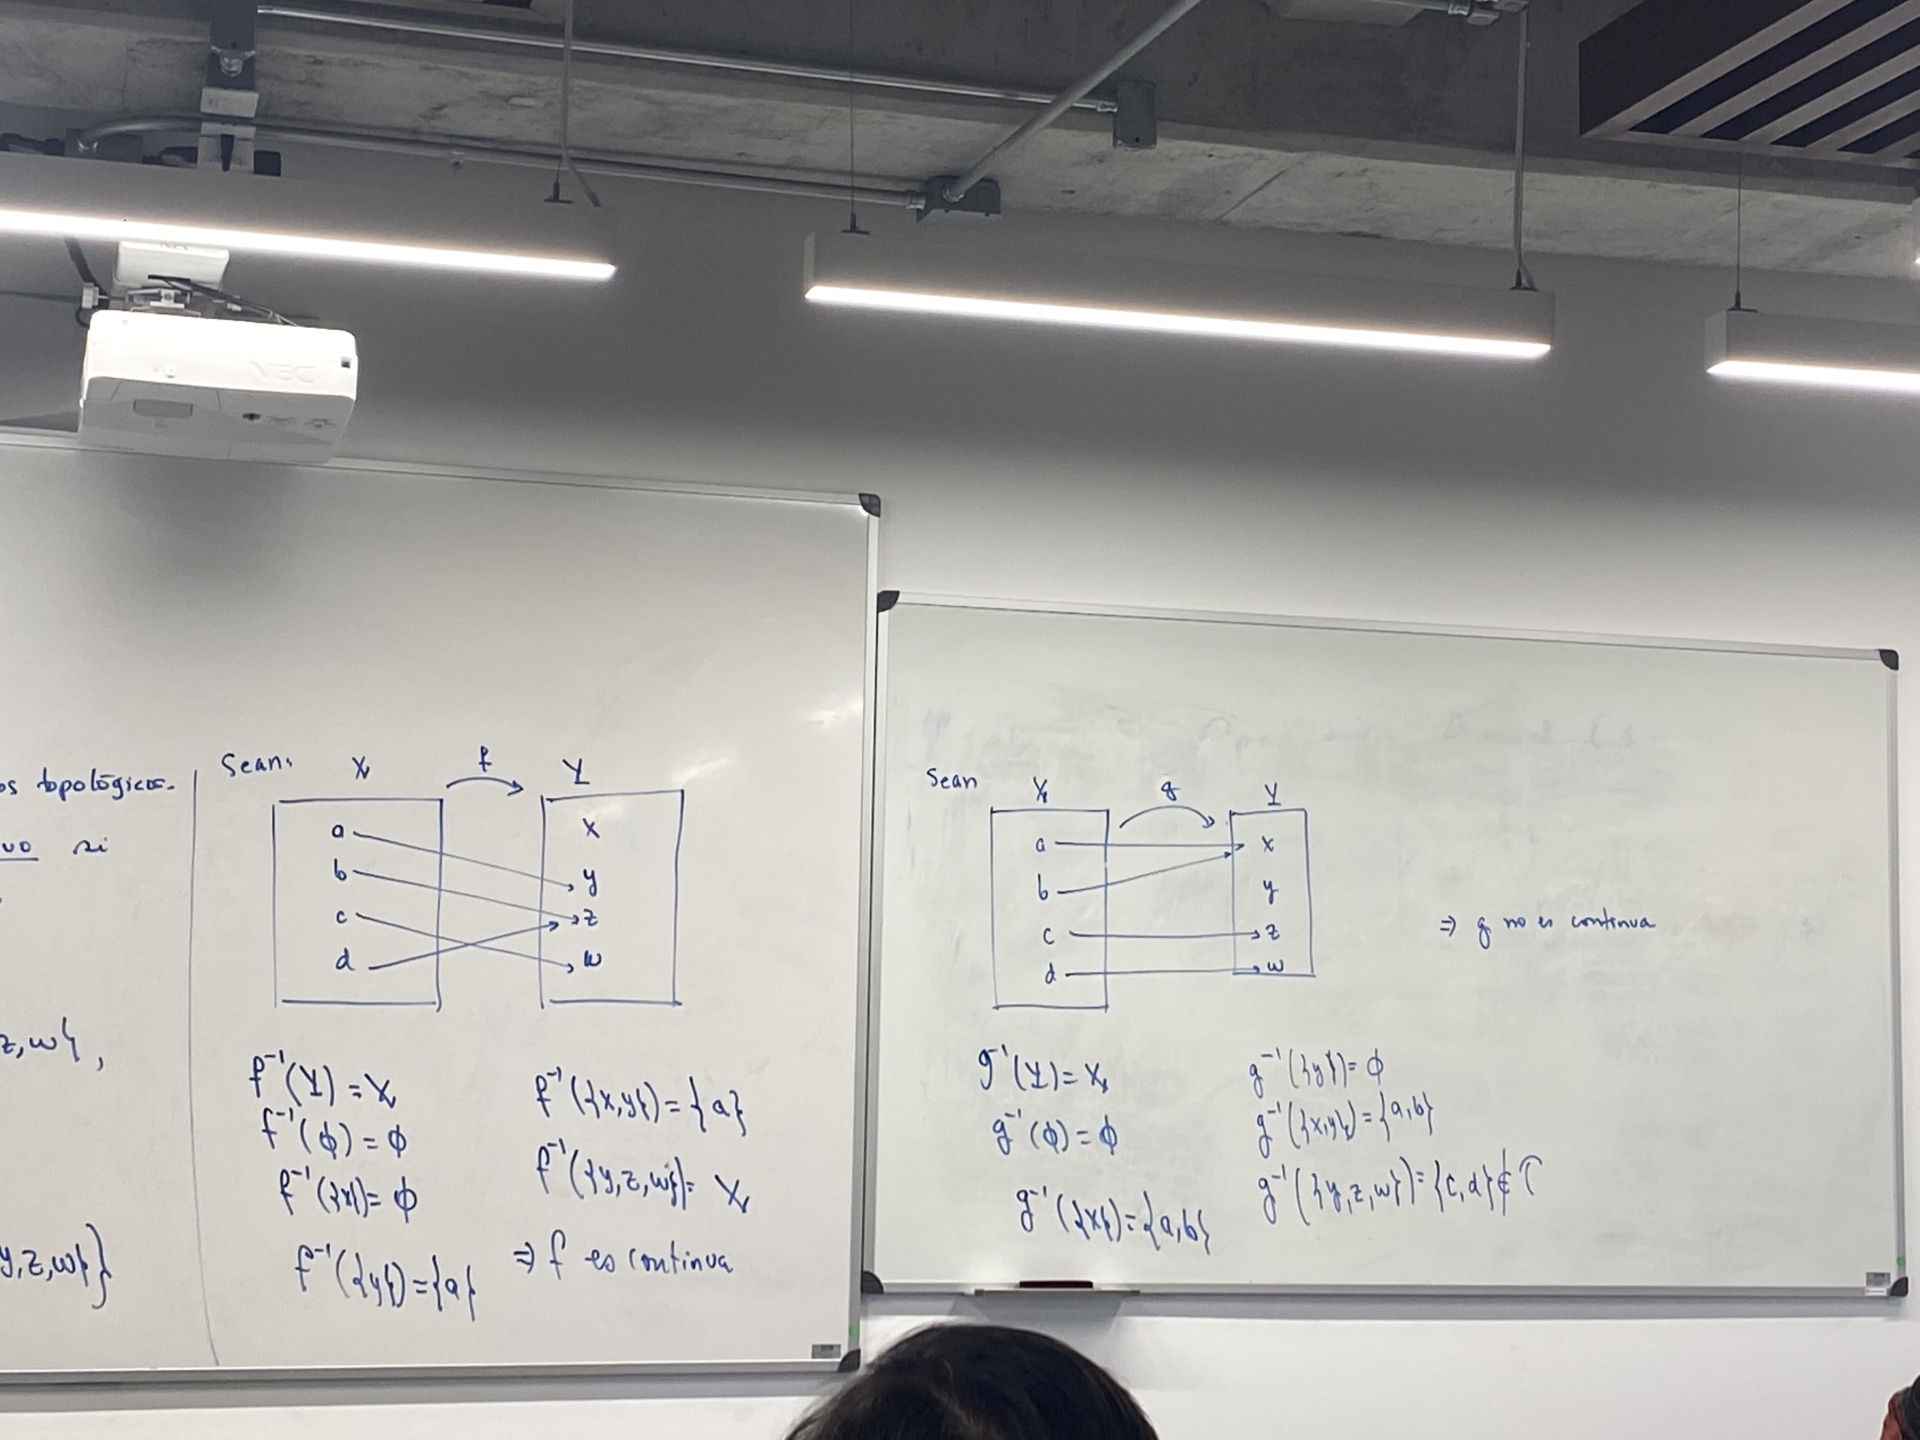
\includegraphics[scale=0.2]{imagenes/ejemplos1.jpeg}
    \end{figure}
\end{ejemplo}

\begin{nota}
    Sea $f: (X,\tau)\to (Y,\tau^*)$ un mapeo y suponga que $\beta=\{B_i\}$ es una base para $\tau^*$. Sea $G\in \tau^*\implies G=\bigcup_{i}B_i,B_i\in\beta $. Entonces, $f^{-1}(G)=g^{-1}\left(\bigcup_iB_i\right)=\bigcup_i f^{-1}(B_i)\implies f^{-1}(G)\in \tau$, si $f^{-1}(B_i)\in \tau$. 
\end{nota}

\begin{nota}
    Dado un mapeo $f:X\to Y$ y si $A\subseteq Y\implies f^{-1}[A^c]=[f^{-1}(A)]^c$. En efecto: Sea $x\in f^{-1}(A^c)\iff f(x)\in A^c \iff f(x)\not\in A\iff x\not\in f^{-1}(A)\iff x\in [f^{-1}(A)]^c$
    
\end{nota}

\begin{nota}
    \begin{enumerate}
        \item Sean $f:(X,\tau)\to(Y,\tau^*)$ un mapeo continuo y sea $F$ un cerrado de $Y\implies f^{-1}(F^c)=\left[f^{-1}(F)\right]^c\in \tau \implies f^{-1}(F)$ es cerrado en $X$.  
        \item Sea $G$ un abierto de $Y\implies G^c$ es cerrado de $Y$. Si $f^{-1}[G^c]=[f^{-1}(G)]^c$ es cerrado, entonces $f^{-1}(G)\in \tau\implies f$ es continuo 
    \end{enumerate}
    
\end{nota}


\begin{prop}
    Sea $f:X\to Y$ un mapeo entre espacios topológicos. Entonces, $f$ es un mapeo continuo ssi $f(\overline{A})\subset \overline{f(A)},\forall A\subseteq X$
    \begin{cajita}
        Propiedades: 
        \begin{enumerate}
            \item $f[f^{-1}(A)]=A$
            \item $f^{-1}[\underbrace{f(A)}_{\subseteq X}]\supset A$
        \end{enumerate}
    \end{cajita}
    \begin{dem}
        Sea
        \begin{itemize}
            \item $(\implies )$ Suponga que $f$ es continuo y sabemos que $f(A)\subset \overline{f(A)}\implies f^{-1}[f(A)]\subset f^{-1}[\overline{f(A)}]$. Además, como $\overline{f(A)}$ es cerrado $\implies f^{-1}[\overline{f(A)}]$ es cerrado (ya que $f$ continuo). Entonces, 
            \begin{align*}
                A\subseteq \underbrace{f^{-1}[\overline{A}]}_{cerrado} &\implies A\subset \overline{A}\subset f^{-1}[\overline{f(A)}]\\
                &\implies f(\overline{A})\subset f[f^{-1}[\overline{f(A)}]]\\
                &\implies f(\overline{A})\subset \overline{f(A)}
            \end{align*}
            \item $(\impliedby)$ Supóngase que $f(\overline{A})\subset \overline{f(A)},\forall A\subseteq X$. Sea $C$ un cerrado de $Y$. Sea $A=f^{-1}(C)\implies f[\overline{f^{-1}(C)}]\subseteq \overline{f(f^{-1}(C))}\implies f[\overline{f^{-1}(C)}]\subseteq C\implies f^{-1}[f[\overline{f^{-1}(C)}]]\subseteq f^{-1}(C)\implies \overline{f^{-1}(C)}\subset f^{-1}(C)\implies f^{-1}(C)\subset \overline{f^{-1}(C)}\subset f^{-1}(C)\implies f^{-1}(C)=\overline{f^{-1}(C)}\implies f^{-1}(C)$ es cerrado. 
        \end{itemize}
    \end{dem}
\end{prop}
